\documentclass[12pt,oneside,english,a4paper]{article}
\usepackage{babel}
\usepackage[utf8]{inputenc}
\usepackage[T1]{fontenc}
\usepackage{color}
\usepackage{graphicx}
\usepackage{wallpaper}
\usepackage{wrapfig,booktabs}

\usepackage{fancyhdr}

\usepackage{fourier-orns}
\newcommand{\dash}{\noindent \newline\textcolor{black}{\hrulefill~ \raisebox{-2.5pt}[10pt][10pt]{\leafright \decofourleft \decothreeleft  \aldineright \decotwo \floweroneleft \decoone   \floweroneright \decotwo \aldineleft\decothreeright \decofourright \leafleft} ~  \hrulefill}}

\usepackage{titlesec}
\titleformat*{\section}{\it\huge\bfseries}
\titleformat*{\subsection}{\it\huge\bfseries}
\titleformat*{\subsubsection}{\it\LARGE\bfseries}
\titleformat*{\paragraph}{\huge\bfseries}
\titleformat*{\subparagraph}{\LARGE\bfseries}

\usepackage[left=20px,right=20px,top=50px,bottom=50px,paperwidth=8in,paperheight=12in]{geometry}


\usepackage[cjk]{kotex}

\usepackage{amsthm} 
\usepackage{amsmath} 
\usepackage{amsfonts}
\usepackage{enumerate} 
\usepackage{cite}
\usepackage{graphics} 
\usepackage{graphicx,lscape} 
\usepackage{subcaption}
\usepackage{algpseudocode}
\usepackage{algorithm}
\usepackage{titlesec}
\usepackage{cite, url}
\usepackage{amssymb}

\def\bk{\paragraph{\LARGE$$}\LARGE}
\def\ck{\paragraph{\LARGE$\bullet$}\LARGE}
\def\pf{\paragraph{\LARGE(pf)}\LARGE}
\def\note{\paragraph{\LARGE\textit{\underline{note:}}}\LARGE}
\def\ex{\paragraph{\LARGE\textit{example:}}\LARGE}
\newcommand{\para}[1]{\paragraph{\LARGE\it\underline{\textbf{#1:}}}\LARGE}
\newcommand{\parablue}[1]{\paragraph{\LARGE\textcolor{blue}{\it\underline{\textbf{#1:}}}}\LARGE}
\newcommand{\parared}[1]{\paragraph{\LARGE\textcolor{red}{\it\underline{\textbf{#1:}}}}\LARGE}
\newcommand{\paraviolet}[1]{\paragraph{\LARGE\textcolor{violet}{\it\underline{\textbf{#1:}}}}\LARGE}
\newcommand{\paraorange}[1]{\paragraph{\LARGE\textcolor{orange}{\it\underline{\textbf{#1:}}}}\LARGE}


\def\one{\paragraph{\large(1)}\LARGE}
\def\two{\paragraph{\LARGE(2)}\LARGE}
\def\three{\paragraph{\LARGE(3)}\LARGE}
\def\four{\paragraph{\LARGE(4)}\LARGE}
\def\five{\paragraph{\LARGE(5)}\LARGE}
\def\six{\paragraph{\LARGE(6)}\LARGE}
\def\seven{\paragraph{\LARGE(7)}\LARGE}
\def\eight{\paragraph{\LARGE(8)}\LARGE}
\def\nine{\paragraph{\LARGE(9)}\LARGE}
\def\ten{\paragraph{\LARGE(10)}\LARGE}

\def\cka{\paragraph{\LARGE(a)}\LARGE}
\def\ckb{\paragraph{\LARGE(b)}\LARGE}
\def\ckc{\paragraph{\LARGE(c)}\LARGE}
\def\ckd{\paragraph{\LARGE(d)}\LARGE}
\def\cke{\paragraph{\LARGE(e)}\LARGE}
\def\ckf{\paragraph{\LARGE(f)}\LARGE}
\def\ckg{\paragraph{\LARGE(g)}\LARGE}
\def\ckh{\paragraph{\LARGE(h)}\LARGE}
\def\cki{\paragraph{\LARGE(i)}\LARGE}
\def\ckj{\paragraph{\LARGE(j)}\LARGE}

\newcommand{\bs}[1]{\mbox{\boldmath $#1$}}

\newcommand{\bsa}{\mbox{\boldmath $a$}}
\newcommand{\bsb}{\mbox{\boldmath $b$}}
\newcommand{\bsc}{\mbox{\boldmath $c$}}
\newcommand{\bsd}{\mbox{\boldmath $d$}}
\newcommand{\bse}{\mbox{\boldmath $e$}}
\newcommand{\bsf}{\mbox{\boldmath $f$}}
\newcommand{\bsg}{\mbox{\boldmath $g$}}
\newcommand{\bsh}{\mbox{\boldmath $h$}}
\newcommand{\bsi}{\mbox{\boldmath $i$}}
\newcommand{\bsj}{\mbox{\boldmath $j$}}
\newcommand{\bsk}{\mbox{\boldmath $k$}}
\newcommand{\bsl}{\mbox{\boldmath $l$}}
\newcommand{\bsm}{\mbox{\boldmath $m$}}
\newcommand{\bsn}{\mbox{\boldmath $n$}}
\newcommand{\bso}{\mbox{\boldmath $o$}}
\newcommand{\bsp}{\mbox{\boldmath $p$}}
\newcommand{\bsq}{\mbox{\boldmath $q$}}
\newcommand{\bsr}{\mbox{\boldmath $r$}}
\newcommand{\bss}{\mbox{\boldmath $s$}}
\newcommand{\bst}{\mbox{\boldmath $t$}}
\newcommand{\bsu}{\mbox{\boldmath $u$}}
\newcommand{\bsv}{\mbox{\boldmath $v$}}
\newcommand{\bsw}{\mbox{\boldmath $w$}}
\newcommand{\bsx}{\mbox{\boldmath $x$}}
\newcommand{\bsy}{\mbox{\boldmath $y$}}
\newcommand{\bsz}{\mbox{\boldmath $z$}}

\newcommand{\bfa}{\mbox{$\bf{a}$}}
\newcommand{\bfb}{\mbox{$\bf{b}$}}
\newcommand{\bfc}{\mbox{$\bf{c}$}}
\newcommand{\bfd}{\mbox{$\bf{d}$}}
\newcommand{\bfe}{\mbox{$\bf{e}$}}
\newcommand{\bff}{\mbox{$\bf{f}$}}
\newcommand{\bfg}{\mbox{$\bf{g}$}}
\newcommand{\bfh}{\mbox{$\bf{h}$}}
\newcommand{\bfi}{\mbox{$\bf{i}$}}
\newcommand{\bfj}{\mbox{$\bf{j}$}}
\newcommand{\bfk}{\mbox{$\bf{k}$}}
\newcommand{\bfl}{\mbox{$\bf{l}$}}
\newcommand{\bfm}{\mbox{$\bf{m}$}}
\newcommand{\bfn}{\mbox{$\bf{n}$}}
\newcommand{\bfo}{\mbox{$\bf{o}$}}
\newcommand{\bfp}{\mbox{$\bf{p}$}}
\newcommand{\bfq}{\mbox{$\bf{q}$}}
\newcommand{\bfr}{\mbox{$\bf{r}$}}
\newcommand{\bfs}{\mbox{$\bf{s}$}}
\newcommand{\bft}{\mbox{$\bf{t}$}}
\newcommand{\bfu}{\mbox{$\bf{u}$}}
\newcommand{\bfv}{\mbox{$\bf{v}$}}
\newcommand{\bfw}{\mbox{$\bf{w}$}}
\newcommand{\bfx}{\mbox{$\bf{x}$}}
\newcommand{\bfy}{\mbox{$\bf{y}$}}
\newcommand{\bfz}{\mbox{$\bf{z}$}}

\newcommand{\bsA}{\mbox{\boldmath $A$}}
\newcommand{\bsB}{\mbox{\boldmath $B$}}
\newcommand{\bsC}{\mbox{\boldmath $C$}}
\newcommand{\bsD}{\mbox{\boldmath $D$}}
\newcommand{\bsE}{\mbox{\boldmath $E$}}
\newcommand{\bsF}{\mbox{\boldmath $F$}}
\newcommand{\bsG}{\mbox{\boldmath $G$}}
\newcommand{\bsH}{\mbox{\boldmath $H$}}
\newcommand{\bsI}{\mbox{\boldmath $I$}}
\newcommand{\bsJ}{\mbox{\boldmath $J$}}
\newcommand{\bsK}{\mbox{\boldmath $K$}}
\newcommand{\bsL}{\mbox{\boldmath $L$}}
\newcommand{\bsM}{\mbox{\boldmath $M$}}
\newcommand{\bsN}{\mbox{\boldmath $N$}}
\newcommand{\bsO}{\mbox{\boldmath $O$}}
\newcommand{\bsP}{\mbox{\boldmath $P$}}
\newcommand{\bsQ}{\mbox{\boldmath $Q$}}
\newcommand{\bsR}{\mbox{\boldmath $R$}}
\newcommand{\bsS}{\mbox{\boldmath $S$}}
\newcommand{\bsT}{\mbox{\boldmath $T$}}
\newcommand{\bsU}{\mbox{\boldmath $U$}}
\newcommand{\bsV}{\mbox{\boldmath $V$}}
\newcommand{\bsW}{\mbox{\boldmath $W$}}
\newcommand{\bsX}{\mbox{\boldmath $X$}}
\newcommand{\bsY}{\mbox{\boldmath $Y$}}
\newcommand{\bsZ}{\mbox{\boldmath $Z$}}

\newcommand{\bfA}{\mbox{$\bf{A}$}}
\newcommand{\bfB}{\mbox{$\bf{B}$}}
\newcommand{\bfC}{\mbox{$\bf{C}$}}
\newcommand{\bfD}{\mbox{$\bf{D}$}}
\newcommand{\bfE}{\mbox{$\bf{E}$}}
\newcommand{\bfF}{\mbox{$\bf{F}$}}
\newcommand{\bfG}{\mbox{$\bf{G}$}}
\newcommand{\bfH}{\mbox{$\bf{H}$}}
\newcommand{\bfI}{\mbox{$\bf{I}$}}
\newcommand{\bfJ}{\mbox{$\bf{J}$}}
\newcommand{\bfK}{\mbox{$\bf{K}$}}
\newcommand{\bfL}{\mbox{$\bf{L}$}}
\newcommand{\bfM}{\mbox{$\bf{M}$}}
\newcommand{\bfN}{\mbox{$\bf{N}$}}
\newcommand{\bfO}{\mbox{$\bf{O}$}}
\newcommand{\bfP}{\mbox{$\bf{P}$}}
\newcommand{\bfQ}{\mbox{$\bf{Q}$}}
\newcommand{\bfR}{\mbox{$\bf{R}$}}
\newcommand{\bfS}{\mbox{$\bf{S}$}}
\newcommand{\bfT}{\mbox{$\bf{T}$}}
\newcommand{\bfU}{\mbox{$\bf{U}$}}
\newcommand{\bfV}{\mbox{$\bf{V}$}}
\newcommand{\bfW}{\mbox{$\bf{W}$}}
\newcommand{\bfX}{\mbox{$\bf{X}$}}
\newcommand{\bfY}{\mbox{$\bf{Y}$}}
\newcommand{\bfZ}{\mbox{$\bf{Z}$}}

\DeclareMathOperator*{\argmin}{argmin} 
\DeclareMathOperator*{\argmax}{argmax} 
\renewcommand{\footnotesize}{\fontsize{9pt}{11pt}\Large}

\usepackage[svgnames]{xcolor}
\usepackage{listings}

\lstset{language=R,
    basicstyle=\LARGE\tt,
    stringstyle=\color{DarkGreen},
    otherkeywords={0,1,2,3,4,5,6,7,8,9},
    morekeywords={TRUE,FALSE},
    deletekeywords={data,frame,length,as,character},
    %keywordstyle=\color{blue},
    commentstyle=\color{DarkGreen},
}
\CJKscale{0.9}
\begin{document}
\section{Weak Ergodicity}
\parared{Theorem A \large{(modified version of Theorem 2 in Hajnal 1958)}} 
For any Markov chain and stopping time $N$, 
\[
[\bsH_n]\leq \prod_{j=1}^{n-1}(1-\{\bsP_j\})[\bsP_n]\leq \prod_{j=1}^{n}(1-\{\bsP_j\}) \quad \mbox{on $n \leq N$.}
\]

From Theorem A we can prove Theorem B. which is upgrade version of Theorem 3 in Hajnal 1958.

\parared{Theorem B \large{(modified version of Theorem 3 in Hajnal 1958)}} 


\parared{Theorem C} Let $N_{\tau}=\inf_\tau\{\tau>N_{\tau-1}: {\cal U}_{\tau}=\emptyset \}$ for all $\tau=1,2,\dots$ with $N_0=0$. Then for all $j=1,2,\dots$ $\{N_j=\infty\}=\emptyset$, i.e., the snow can't flow infinitely.

\para{proof} Let $M_j=N_{j+1}-N_j$. It is sufficient to show that $\{M_j=\infty\}=\emptyset$ for all $j=0,1,2,\dots$. 
%We begin with the case that $f(v_1)=\dots=f(v_n)=0$. 
Suppose $M_0=\infty$, i.e., the snow is "never blocked". Denote the $v^{\tau}_{(1)},\dots,v^{\tau}_{(n)}$ as the ordered index by value of $h^{\tau}_1,\dots,h^{\tau}_n$, i.e., 
\[
h_{v_{(1)}^{\tau}}^{\tau} \leq \dots \leq h_{v_{(n)}^{\tau}}^{\tau}.
\]
Let $R_\tau=1-\prod_{k=1}^{n}I(v_{(k)}^{\tau}=v_{(k)}^{\tau+1})$. Thus $R_{\tau}=0$ means that there is no changes in shape of land. Suppose that $\sum_{\tau=1}^{\infty}R_{\tau}=0$, this means that there is no reversal in all $\tau$. For all $i=1,2,\dots,n$, let $N^{*}(v_i)=\inf_{\tau}\{\tau>0: T_\tau=v_i \}$. Clearly, $N^*({v_{(1)}^0})<\infty$. The assumption $\sum_{\tau=1}^{\infty}R_\tau=0$ implies that $h^{\tau}(v_{(1)}^0)\leq \min_v h_v^{\tau}$ for all $\tau$. This means that snow is "blocked" at least at $\tau=N^*(v_{(1)}^0)$ (of course it could be faster), and it makes contradiction. Now suppose $\sum_{\tau=1}^{\infty}R_{\tau}<\infty$. Then there exists $L$ such that $\sum_{\tau=L+1}^{\infty} R^{\tau} =0$. Thus it makes contradiction again. Now suppose that $\sum_{\tau=1}^{\infty} R^\tau=\infty$. Then there exist $u,v \in V$ such that sign of $h^{\tau}_u-h^{\tau}_v$ changes infinitely often. Denote $C_k$ be the $k$-th sign change of $h^{\tau}_u-h^{\tau}_v$, i.e., 
\[
C_k=\inf_{\tau}\Big\{\tau>C_{k-1}: \big(h^{\tau-1}_u-h^{\tau-1}_v\big)\big(h^{\tau}_u-h^{\tau}_v\big)<0 \Big\}
\]
with $C_0=0$. Denote $\Delta_k=|h_u^{C_k}-h_v^{C_k}|$ and $\Delta_k^-=|h_u^{C_k-1}-h_v^{C_k-1}|$. 

\para{Claim A} For all $k=1,2,\dots,$ there exists $C(k)$ such that $C_{k}\leq C(k) < C_{k+1}$ and 
\[
b\gamma^{C(k)}-b\gamma^{C_{k+1}}<\left|h_u^{C(k)-1}-h_v^{C(k)-1} \right|\leq \Delta_k.
\]
\proof asdf. 

\para{Claim B} For all $k=1,2,\dots,$ there exist $C(k)$ such that $C_k<C(k)<C_{k+1}$ and 
\[
\gamma^{C(k)}<2\gamma^{C_{k+1}}
\]
\proof sdf 

\para{Claim C} There exists $\kappa_0$ such that 
\[
\min(\Delta_{\kappa_0}^-,\Delta_{\kappa_0}) < \min(\Delta_{\kappa_0+1}^-,\Delta_{\kappa_0+1})
\]
\proof sdf

\para{Claim D} For all $\epsilon>0$ there exists $\kappa_1$ such that 
\[
\frac{\left|h_u^{C(\kappa_1)-1}-h_v^{C(\kappa_1)-1} \right|}{b\gamma^{C_{\kappa_1+1}}} <\epsilon
\]
\proof sdf

\bk For all $k$, there exists $m$ such that  
\[
m>C_k\quad\mbox{and}\quad \left|h_u^{C(m)-1}-h_v^{C(m)-1} \right|< b\gamma^{C_{k}}-b\gamma^{C_{m+1}}
\]
By Claim A, we have 
\[
b\gamma^{C(m)}-b\gamma^{C_{m+1}}<b\gamma^{C_{m+1}}\epsilon
\]
Thus 
\[
1-\gamma^{C_{m+1}-C(m)}<\epsilon
\]
Since $\epsilon$ is arbitary, it makes contradiction. 

\dash 

Then $\Delta_1=\Delta_1^-$ Choose $C_k$ such that 
\[
b\gamma^{C_{k}}<\min(\Delta_1^-,\Delta_1)
\]
From Lemma A and $\Delta_1+\Delta_1^-=b\gamma^{C_1}$, we have 
\[
b\gamma^{C(k)}-\left|h_u^{C(k)-1}-h_v^{C(k)-1} \right|<\min(\Delta_1^-,\Delta_1)
\]

\parared{Theorem D} Let ${\cal G}=(V,{\boldsymbol E},{\boldsymbol W})$ be a weighted graph with $|V|=n$ and $f$ be a graph signal defined on ${\cal G}$. Let ${\cal H}(f,{\cal G};\tau)$ denote the heavy snow transformation of $f$. 
Let $\{T_\tau\}$ as trace of snow with $p^{\tau}_{u,v}$. Then $\{T_{\tau}\}$ is \emph{ergodic in the weak sense}, i.e., as $\tau \to \infty$
\[
\left |p_{u,v}^{(\ell,\tau)}-p_{u',v}^{(\ell,\tau)}\right| \to 0 \quad \mbox{for any $\ell$ and all $u,u',v$.}
\]
where $p_{u,v}^{(\ell,\tau)}$ is $(u,v)$-th element of ${\bs P}_{\ell}{\bs P}_{\ell+1}\dots{\bs P}_{\ell+\tau}$.

\proof 
Let $$\{\bsP\}=\min_{u,u'}\sum_{v}\min(p_{u,v},p_{u'v}).$$%. and $$[\bsP]=\max_v\max_{u,u'}\left|P_{u,v}-P_{u',v}\right|$$
Denote $N_{\tau}=\inf_\tau\{\tau>N_{\tau-1}: {\cal U}^{\tau}=\emptyset \}$ for all $\tau=1,2,\dots$ with $N_0=0$. Let $M_j=N_{j+1}-N_j$. Note that $N_0,N_1,N_2,\dots$ and $M_0,M_1,M_2,\dots$ is stopping time. Due to Theorem C, we can devide the set $\{0,1,2,3,\dots,\}$ into infinitely many partition such that 
\[
\{0,\dots,N_1-1\}, \{N_1,\dots,N_2-1\}, \{N_2,\dots,N_3-1\}, \dots
\]
Define $\bsP_{(N_j,M_j)}=\bsP_{N_j}\dots \bsP_{N_{j+1}-1}$ From Theorem B, it suffices to show that $\sum_{j=0}^{\infty}\left\{{\bsP}_{(N_j,M_j)} \right\}$
diverges. By Lemma 1 in Hajnal (1958)
\[
\left\{\bsP_{(N_j,M_j)}\right\}\geq\left\{\bsP
_{N_j}\right\}=1\quad \mbox{for all $j=0,1,2\dots,$}
\]
Thus theorem is proved.


%Clearly $h_u^{C_1-1}+b\gamma^{C_1}>h_v^{C_1-1}$. $h_u^{C_2-1}>h_v^{C_2-1}$. 

%For all $i=1,2,\dots,n$, let $N_i^{*}=\inf_{\tau}\{\tau>0: T^\tau=v_i \}$ and $N_i^{**}=\inf_{\tau}\{\tau>N_i^*:T^\tau=v_i\}$. Denote the time of the first revisit of all nodes as $N^{**}$, i.e., $N^{**}=\min\{N_1^{**},\dots,N_n^{**}\}$. Further denote the node where snow stays at $N^{**}$ as $\tilde{v}$, i.e., $\tilde{v}=T^{N^{**}}$. Now define $N^{*}=\inf_{\tau}\{\tau>0:T^\tau =\tilde{v}\}$ which is the first visiting time of node $\tilde{v}$. From $M_0=\infty$ we have $N^*,N^{**} <\infty$ since we assume the finite Markov chain. Clearly, $$h_{\tilde{v}}^{N^*}=b\gamma^{N^*}>\max_{N^*<\tau<N^{**}}\max_v h_v^{\tau}\geq \max_{v \in {\cal N}_{\tilde v}}h_{\tilde v}^{N^{**}-1}$$ and this means that the snow is "blocked" when $N^{**}-1$. It makes contradictions.


\dash
\section{Example 1}
쌓인눈 변환의 결과로 얻어지는 $\bsW(\tau)$을 고려하자. 이 매트릭스의 colsum을 $d_i(\tau)$이라고 하자. 따라서 $d_i(\tau)$는 어디에서 시작했는지 모르겠지만 노드 $i$로 도착할 확률의 합을 의미한다. 이를 이용하여 아래와 같은 행벡터를 만든다. 
\[
\bsd(\tau)=[d_1(\tau),\dots,d_n(\tau)]
\]
이제 $\bsd$를 이용하여 
$
\alpha_i(\tau)=\frac{d_i(\tau)}{d_1(\tau)+\dots+d_n(\tau)}
$
와 같은 확률을 정의하자. 그리고 
\[
\bs{\alpha}(\tau)=[\alpha_1(\tau),\dots, \alpha_n(\tau)]\]
와 같은 행벡터를 생각하자. 즉 $\bs{\alpha}(\tau)$는 $\bsW(\tau)$의 columsum을 구해서 $\bsd(\tau)$와 같은 행벡터를 만들고 $\bsd(\tau)$를 표준화하여 얻을 수 있다. 

\ck 정규그래프에서 $\bs{\alpha}(\tau)=\bs{\pi}(\tau)$임을 보이자. 


\para{proof}
\ck $e^{-x} \geq 1-x $이므로 $W_{12}^{\tau}=e^{-\frac{\Sigma_{12}^\tau}{2(\theta_n^\tau)^2}}\geq 1-\frac{\Sigma_{12}^\tau}{2(\theta_n^\tau)^2}$가 성립한다. 따라서 아래가 성립한다. 그다지 큰 의미는 없는듯. 
\begin{align*}
& W_{11}^{\tau}+\dots+W_{1n}^{\tau} 
\geq (n-1)-\frac{1}{2(\theta_n^\tau)^2}\big(\Sigma_{12}^{\tau}+\dots+\Sigma_{1n}^{\tau}\big)
\end{align*}

\ck 고정된 $i$에 대하여 수열 $\big\{\pi_i^{\tau}-\pi_i^{\tau-1}\big\}$은 코시수열임을 보이자. 즉 아래를 보이면 된다. 
\[
\pi_i^{\tau}-\pi_i^{\tau-1}=\frac{d_i^{\tau}}{d_1^{\tau}+\dots+d_n^{\tau}}-\frac{d_i^{\tau-1}}{d_1^{\tau-1}+\dots+d_n^{\tau-1}}=o(1)
\]
따라서 아래를 보이면 된다. 
\[
\frac{d_i^{\tau}}{d_1^{\tau}+\dots+d_n^{\tau}}=\frac{d_i^{\tau-1}}{d_1^{\tau-1}+\dots+d_n^{\tau-1}}+o(1)
\]

\parablue{case1} : $d_1^{\tau}+\dots+d_n^{\tau}=d_1^{\tau-1}+\dots+d_n^{\tau-1}$이라고 하자. 
\ck 아래를 보이기만 하면 된다. 
\[
d_i^{\tau}-d_i^{\tau-1}=o(1)
\]
그런데 
\[
d_i^{\tau}=W_{i1}^{\tau}+W_{i2}^{\tau}+\dots+W_{in}^{\tau}=W_{i2}^{\tau}+\dots+W_{in}^{\tau}
\]
이므로 아래를 보이면 된다. 
\[
(W_{i1}^{\tau}-W_{i1}^{\tau-1})+\dots+(W_{in}^{\tau}-W_{in}^{\tau-1})=o(1)
\]
결국 모든 $j$에 대하여 아래를 보이면 된다. 
\[
W_{ij}^{\tau}-W_{ij}^{\tau-1}=o(1)
\]
따라서 아래를 보이면된다. 
\[
\frac{W_{ij}^{\tau}}{W_{ij}^{\tau-1}}-1=o(1)
\]

\note 
아래를 관찰하자. 
\begin{align*}
W_{ij}^{\tau}&=e^{-\frac{\Sigma_{ij}^{\tau}}{2(\theta_n^{\tau})^2}}
=e^{-\frac{1}{2}\big(\frac{h_i^0-h_j^0}{\theta_n^{\tau}}\big)^2}
e^{-\frac{1}{2}\big(\frac{h_i^1-h_j^1}{\theta_n^{\tau}}\big)^2}
\dots
e^{-\frac{1}{2}\big(\frac{h_i^{\tau-1}-h_j^{\tau-1}}{\theta_n^{\tau}}\big)^2}
e^{-\frac{1}{2}\big(\frac{h_i^\tau-h_j^\tau}{\theta_n^{\tau}}\big)^2} \\
W_{ij}^{\tau-1}&=e^{-\frac{\Sigma_{ij}^{\tau-1}}{2(\theta_n^{\tau-1})^2}}
=e^{-\frac{1}{2}\big(\frac{h_i^0-h_j^0}{\theta_n^{\tau-1}}\big)^2}
e^{-\frac{1}{2}\big(\frac{h_i^1-h_j^1}{\theta_n^{\tau-1}}\big)^2}
\dots
e^{-\frac{1}{2}\big(\frac{h_i^{\tau-1}-h_j^{\tau-1}}{\theta_n^{\tau-1}}\big)^2}
\end{align*}

\ck 따라서 
\[
\frac{W_{ij}^{\tau}}{W_{ij}^{\tau-1}}
=A_1 \times \dots \times A_{\tau-1}\times A_\tau
\]
이때 
\begin{align*}
A_0&=\exp\left(-\frac{1}{2}\left(\frac{1}{(\theta_n^\tau)^2}-\frac{1}{(\theta_n^{\tau-1})^2}\right)(h_i^0-h_j^0)^2\right) \\
A_1&=\exp\left(-\frac{1}{2}\left(\frac{1}{(\theta_n^\tau)^2}-\frac{1}{(\theta_n^{\tau-1})^2}\right)(h_i^1-h_j^1)^2\right) \\
\dots \\
A_{\tau-1}&=\exp\left(-\frac{1}{2}\left(\frac{1}{(\theta_n^\tau)^2}-\frac{1}{(\theta_n^{\tau-1})^2}\right)(h_i^{\tau-1}-h_j^{\tau-1})^2\right) \\ 
A_{\tau}&=\exp\left(-\frac{1}{2}\frac{1}{(\theta_n^\tau)^2}(h_i^{\tau}-h_j^{\tau})^2\right)
\end{align*}

\one 그런데 
\[
\frac{1}{(\theta_n^\tau)^2}-\frac{1}{(\theta_n^{\tau-1})^2}=o(1)
\]
이다. 왜냐하면 $\left\{\frac{1}{(\theta_n^{\tau})^2}\right\}_{\tau=1}^{\infty}$이 수렴하는 수열이기 때문이다. (수렴하는 수열은 코시수열임) 
\two 또한 모든 $\tau$에 대하여 
\[
\max_{i,j}|h_i^{\tau}-h_j^{\tau}|=O(1)
\]
이다. (한쪽에만 눈이 쌓일수는 없음.) 
\three $\exp$가 연속함수이므로 $A_1,\dots,A_{\tau-1}$는 모두 $1$로 수렴한다. 그리고 $A_{\tau}$ 역시 $1$로 수렴한다.

\ck 따라서 
\[
\frac{W_{ij}^{\tau}}{W_{ij}^{\tau-1}}
=1+o(1)
\]

\parablue{case2} :  이제 $d_1^{\tau}+\dots+d_n^{\tau}\neq d_1^{\tau-1}+\dots+d_n^{\tau-1}$ 라고 하자. 아래를 정의하자. 
\begin{align*}
&d^{\tau-1}=d_1^{\tau-1}+\dots+d_n^{\tau-1} \\
&d^{\tau}=d_1^{\tau}+\dots+d_n^{\tau} \\
& \tilde{d}^{\tau}=\max(d^{\tau},d^{\tau-1})
\end{align*}
Clearly,
\[
\tilde{d}^{\tau}=O(1)
\]
따라서 case1 을 반복하면 증명이 된다. 



\parared{prop} Let ${\cal G}=(V,{\boldsymbol E},{\boldsymbol W})$ be a weighted graph with $|V|=n$ and $f$ be the graph function defined on ${\cal G}$. Assume that ${\cal G}$ is a regular graph. Suppose that $f(v_1),\dots,f(v_n)$ is $i.i.d$ random sample. Let ${\cal G}^{\tau}=(V,{\boldsymbol E},{\boldsymbol W}^{\tau})$ be the weighted graph induced by the heavy snow transformation of $f$ ${\cal H}(f,{\cal G}; \tau)$. Then we have ${\boldsymbol W}^{\tau} \overset{p}{\to} {\boldsymbol W}$ element-wisely as $\tau \to \infty$.

\proof Using the results in Appendix A.2, we obtain $W_{ij}^{\tau} \sim N(T_{ij}(F),V_{ij}(T,F)/n)$, where $T_{ij}(F):=\int W_{ij}^{\tau}dF^{\tau}$. Note that $T_{ij}(F^{\tau}) \to 1 $ as $\tau \to \infty$ for $i\neq j$ and $T_{ij}(F^{\tau})=0$ for $i=j$. Further, we get $V_{ij}(T,F^{\tau})/n \to 0$ as $\tau \to \infty$ for all $i,j$. Thus ${\boldsymbol W}^{\tau} \overset{p}{\to} {\boldsymbol W}$ element-wisely as $\tau \to \infty$.

\parablue{Appendix 2}:
Let ${\cal G}=(V,{\boldsymbol E},{\boldsymbol W})$ be a weighted graph with $|V|=n$ and $f$ be a graph signal defined on ${\cal G}$. Assume that ${\cal G}$ is a regular graph. Suppose that $f(v_1),\dots,f(v_n)$ is $i.i.d$ random sample. Let ${\cal H}(f,{\cal G}; \tau)$ be the heavy snow transformation of $f$. Since $f(v_i)$ is $i.i.d.$ random variable, ${\boldsymbol h}_i$ is $i.i.d.$ random vector with 
$
{\boldsymbol h}_1^{\tau},\dots,{\boldsymbol h}_n^{\tau} \sim F^{\tau}.
$ 
Define a functional $T(F^{\tau})$ as 
$
T(F^{\tau}):=\int g({\boldsymbol h}) dF^{\tau}.
$
Let $F_n^{\tau}$ be an empirical distribution function of ${\boldsymbol h}_1^{\tau},\dots,{\boldsymbol h}_n^{\tau}$ defined as  
\[
F_n^{\tau}(m) :=\frac{1}{n}\sum_{i=1}^{n}1({\boldsymbol h}^{\tau}_i\leq t).
\]
From Glivenko-Cantelli Lemma,  we obtain $F_n^{\tau} \to F^{\tau}$. Thus, for a sufficiently large $n$, we can say that $F_n^{\tau}$ is a neighborhood of $F^{\tau}$. Hence, we have 
\begin{align*}
T(F_n^{\tau}) & \approx  T(F^{\tau})+\int IF(\boldsymbol{h}^{\tau},T,F^{\tau})d(F_n^{\tau}-F^{\tau}) \\
& = T(F^{\tau})+\int IF(\boldsymbol{h}^{\tau},T,F^{\tau}) dF_n^{\tau}, 
\end{align*}
where $IF({\boldsymbol h}^{\tau}; T,F^{\tau})= \lim_{t\downarrow 0}\frac{T((1-t)F^{\tau} + t \delta(\boldsymbol{h}) )-T(F^{\tau})}{t}$ is an influence function of $T$. Here, $\int IF(\boldsymbol{h}^{\tau},T,F^{\tau})dF^{\tau}=0$ is used. Therefore, it follows that  
\[
\sqrt{n}\Big(T(F_n^{\tau})-T(F^{\tau}) \Big) \to N(0,V(T,F^{\tau})), 
\]
where $V(T,F^{\tau})=\int IF(\boldsymbol{h}^{\tau},T,F^{\tau})^2 dF^{\tau}$. 

\subsection{약간의 수정}
\one $\Sigma_{ij}^{\tau}=\|\bsh_i^{\tau}-\bsh_j^{\tau}\|_2^2=\sum_{\ell=0}^{\tau}(h_i^\ell-h_j^\ell)^2$
\two $h_i^{\tau}=h_i^{\tau-1}+\xi_i^{\tau}$
\three $W_{ij}^{\tau}=\begin{cases}\exp\big(-\frac{1}{2}\frac{\Sigma_{ij}^{\tau}}{(\theta_n^{\tau})^2}\big) & i\neq j \\ 0 & i=j \end{cases}$
\note $\theta_n^{\tau}$은 어떤개념? $\big\{\Sigma_{ij}^{\tau}-{\tt mean}(\Sigma_{ij}^{\tau})\big\}_{i,j}$의 sample variance로 생각하고 
싶은데 애매함. 

\four $d_i^{\tau}=\sum_{j=1}^{n}W_{ij}^{\tau}$. 

\note $d_i^{\tau}:=\mbox{$i$-th 노드와 연결된 weight들의 총합}$
\note $d_i^{\tau}$값이 클수록 $i$-th 노드가 클러스터의 중심부에 있음을 의미함. 

\five $\pi_i^{\tau}:=\frac{d_i^{\tau}}{\sum_{i}^nd_i^{\tau}}$.


\note $\pi_i^{\tau}$는 전체를 1로 보았을때 $i$-번째값이 전체중에서 얼마나 비유사한 아이인지 판단함. (값이 작을수록 비유사하다) 만약에 총 100개의 점이 있다고 하자. $\pi_i^{\tau}=\frac{1}{100}$이라면 일단 평균정도 중요하다는 의미임. 아웃라이어일수록 $\pi_i^{\tau}\approx 0$임. 

\parablue{Theorem} 고정된 $n$에 대하여 
\begin{enumerate}[(i)]
\item $\theta_n^{\tau} \to \infty\quad as\quad \tau \to \infty$
\item $\max_{i,j}|f(v_i)-f(v_j)|=O(1)$
\end{enumerate}
이라면 아래를 만족하는 $\pi^{\star}$가 항상 존재한다. 
\[
\|\bs{\pi}-\bs{\pi}^{\star}\|_2^2=o(1)
\]

\subsection{수정할것들}
\parared{thm} (1) $\cal G=(V,\bsE,\bsW)$를 모든 엣지가 연결된 레귤러 그래프라고 하자. 즉 $\bsW=\bsJ-\bsI$. (2) $f_1,\dots f_{100} \overset{iid}{\sim} N(\mu_1,1)$. 그러면 아래가 성립한다. 
\[
\bsW^{\tau} \overset{p}{\to} \bsJ-\bsI
\]

\parared{thm} (1) $\cal G=(V,\bsE,\bsW)$를 모든 엣지가 연결된 레귤러 그래프라고 하자. 즉 $\bsW=\bsJ-\bsI$. (2) $f_1,\dots f_{50} \overset{iid}{\sim} N(\mu_1,1)$ and $f_{51},\dots,f_{100} \overset{iid}{\sim} N(\mu_2,1)$. 그러면 아래가 성립한다. 
\[
\bsW^{\tau} \overset{p}{\to} \begin{bmatrix}\bsJ-\bsI & \bf{0} \\ \bf{0} & \bsJ-\bsI \end{bmatrix}
\]

\section{MCU 예제에 대한 백업}
\parared{thm} 눈을 쌓을수록 노드정보를 상실한다. HST는 노드정보와 그래프도메인에서의 정보를 연속적으로 변화시키는 장치이다. 
\note 단순히 노드에서의 거리와 그래프도메인의 거리를 가중평균한것과 무슨 차이일까? 

\parared{Theorem C} Suppose that $\max_{i,j}|f(v_i)-f(v_j)|<\infty$. Then for all $i,j$, 
\[
p_{ij}^{\tau} = \frac{W_{ij}}{\sum_{k=1}^{n}W_{ik}}+o(1).
\]
Here
\begin{align*}
& p_{ij}^\tau:=\mbox{Prob}(T^{\tau}=j|T^{\tau-1}=i) \\ 
&=
\begin{cases}
\frac{d(v_j)}{\sum_{k=1}^{n}d(v_k)} & {\cal U}^{\tau-1}=\emptyset \\ 
\frac{1}{|{\cal U}^{\tau-1}|} & ({\cal U}^{\tau-1} \neq \emptyset \mbox{ and})~ v_j \in {\cal U}^{\tau-1}\\ 
0 & {\cal U}^{\tau-1} \neq \emptyset \mbox{ and } v_j \notin {\cal U}^{\tau-1}
\end{cases}
\end{align*}
\proof
For fixed $i,j$, $p_{ij}^{\tau}$ can be expressed as 
\begin{align*}
p_{ij}^{\tau}=I({\cal U}^{\tau-1}=\emptyset)\times \frac{d(v_j)}{\sum_{k=1}^{n}d(v_k)}+I({\cal U}^{\tau-1}\neq \emptyset)\times \frac{I(v_j\in{\cal U}^{\tau-1})}{|{\cal U}^{\tau-1}|}
\end{align*}
Here the left term means the probability that snow blocked at $\tau-1$ and then (randomly) fall down to $v_j$ at $\tau$, and right term means the probability that snow flow from $v_i$ to $v_j$. 

\para{claim 1} $\frac{I(v_j\in{\cal U}^{\tau-1})}{|{\cal U}^{\tau-1}|}=\frac{d(v_j)}{\sum_{k=1}^{n}d(v_k)}+o_p(1)$.

\proof to be showed

\bk From claim 1, we have 
\begin{align*}
p_{ij}^{\tau}&=I({\cal U}^{\tau-1}=\emptyset)\times \frac{d(v_j)}{\sum_{k=1}^{n}d(v_k)}\\ 
&\quad+I({\cal U}^{\tau-1}\neq \emptyset)\times \left(\frac{d(v_j)}{\sum_{k=1}^{n}d(v_k)}+o_p(1)\right)\\
=
\end{align*}


그런데 $\frac{I(v_1\in{\cal U}^{\tau-1})}{|{\cal U}^{\tau-1}|}=\frac{d(v_1)}{d}+o_p(1)$ 이므로 $b^{\tau}=I({\cal U}^{\tau-1}\neq \emptyset)\frac{d(v_1)}{d}+o_p(1)$ 이다. 정리하면
\begin{align*}
& a^{\tau} =I({\cal U}^{\tau-1}=\emptyset)\frac{d(v_2)}{d} \\
& b^{\tau} = I({\cal U}^{\tau-1}\neq\emptyset)\frac{d(v_1)}{d}+o_p(1)
\end{align*}
따라서 만약에 $d(v_1)=d(v_2)$라면 
\[
p_{12}^{\tau}=a^{\tau}+b^{\tau}=\frac{d(v_1)}{d}+o_p(1)=\frac{d(v_2)}{d}+o_p(1)
\]
그런데 $\frac{d(v_2)}{d}=\frac{W_{12}}{\sum_jW_{1j}}$이므로 증명끝. 


\dash 

\section{예제2에 대한 백업 (1)}
\subsection{regular graph에서의 성질}
\parared{Theorem} ${\cal G}=(V,\bsE,\bsW)$가 $k-regular$ 그래프라고 하자. 그리고 $f(v_i)=0$이라고 하자. 그러면 모든 고정된 $i, j,\ell=1,2,\dots,\tau$에 대하여 아래가 성립한다.
\[
p_{ij}^{\ell}=\frac{1}{k}
\]

\subsection{regular graph에서의 성질, 링내에서는 빨-보가 유지된다.}
\ck 빨주노초파남보의 7개의 노드가 있다고 하자. 즉 $V=\{1,2,3,\dots,7\}$이라고 하자. 

\ck 이들은 서로 링형태로 연결되어 있다고 하자. 

\para{주장 1}: $\ell=2$에서 아래가 성립한다.
\[
\Sigma_{13}^{\ell}-\Sigma_{12}^{\ell}\geq 0
\]
등호는 

\para{주장 1의 증명:}
\parared{경우1} 먼저 $\ell=1$에서 노드1에 눈이 있다고 가정하자. (1) 먼저 눈이 노드1에서 블락되었다고 가정하자. $\Longrightarrow$ 이런 경우는 없다. (2) 눈이 노드1에서 2로 흘렀다고 가정하자. 그러면 
\begin{align*}
\Sigma_{12}^{\ell}&=b^2+(1-\gamma)^2b^2 \\
\Sigma_{13}^{\ell}&=2b^2
\end{align*}
이므로 
\[
\Sigma_{13}^{\ell}-\Sigma_{12}^{\ell}=\big(1-(1-\gamma)^2\big)b^2>0
\]
(3) 눈이 노드1에서 7로 흘렀다고 가정하자. 즉 노드1에서 노드2,3을 제외한 다른이웃으로 흘렀다고 가정하자. 그러면 
\[
\Sigma_{13}^{\ell}=\Sigma_{12}^{\ell}
\]
이다. 따라서 경우 1에서는 아래가 성립한다. 
\[
\Sigma_{13}^{\ell}\geq\Sigma_{12}^{\ell}
\] 

\parared{경우2} $\ell=1$에서 노드2에 눈이 있다고 가정하자.
(1) 노드2에서 블락될경우는 없다. (2) 노드2에서 노드1로 흐르는 경우에는 아래와 같다. 
\begin{align*}
\Sigma_{12}^{\ell}&=b^2+(1-\gamma)^2b^2 \\
\Sigma_{13}^{\ell}&=\gamma^2b^2
\end{align*}
이때는 보는것처럼 $\Sigma_{13}^{\ell}<\Sigma_{12}$ 이다. (3) 노드2에서 노드3으로 흐르는 경우는 아래와 같다. 
\begin{align*}
\Sigma_{12}^{\ell}&=2b^2 \\
\Sigma_{13}^{\ell}&=\gamma^2b^2
\end{align*}
이때는 보는것처럼 $\Sigma_{13}^{\ell}>\Sigma_{12}$ 이다. (4) 노드2에서 노드1,3이외에 다른 이웃으로 흐르는 경우는 항상 $\Sigma_{13}^{\ell}=\Sigma_{12}^{\ell}$이다. 따라서 차이는 항상 $0$ 이다. 이제 (2)와 (3)이 같은 확률 $p^{\bigstar}$로 일어난다는 것을 고려하여보자. (Access time이 같다고 하자.) 그러면 평균적으로는 아래와 같이 차이난다. 
\[
E(\Sigma_{13}^{\ell}-\Sigma_{12}^{\ell})=p^{\bigstar}\left[2\gamma^2-3-(1-\gamma)^2 \right]b^2=(\gamma^2+2\gamma-4)p^{\bigstar}b^2
\]

\parared{경우3} $\ell=1$에서 노드3에 눈이 있다고 하자. (1) 노드3에서 블락되는 경우는 없다. (2) 노드3에서 2로 흘렀다고 하자. 이 확률은 $p^{\bigstar}$이다. 
\begin{align*}
\Sigma_{12}^{\ell}&=\gamma^2b^2 \\
\Sigma_{13}^{\ell}&=2b^2
\end{align*}
(3) 노드3에서 1로 흐를수는 없다. (4) 노드3에서 1,2를 제외한 이웃으로 흘렀다고 하자. (이 확률은 $(1-p^{\bigstar})$ 임)
\begin{align*}
\Sigma_{12}^{\ell}&=2b^2 \\
\Sigma_{13}^{\ell}&=2b^2
\end{align*}
따라서 평균적으로 
\[
E(\Sigma_{13}^{\ell}-\Sigma_{12}^{\ell})=\big(4-2(1-p^{\bigstar})-p^{\bigstar}\gamma^2 \big)b^2=(2+(2-\gamma^2)p^{\bigstar})b^2
\]

\ck 경우2와 3을 종합하면 평균적으로 
\[
\big(2+(\gamma^2+2\gamma-4+2-\gamma^2)p^{\bigstar}\big)b^2
=\big(2+(2\gamma-2)p^{\bigstar}\big)b^2\geq 0
\]

\parared{경우4} $\ell=1$에서 노드4에 눈이 있다고 가정하자. 
\[
\Sigma_{13}^{\ell}\geq\Sigma_{12}^{\ell}=0
\]

\para{경우5} $\ell=1$에서 노드5에 눈이 있다고 가정하자. 
\[
\Sigma_{13}^{\ell}=\Sigma_{12}^{\ell}=0
\]
\para{경우6} $\ell=1$에서 노드6에 눈이 있다고 가정하자. 
\[
\Sigma_{13}^{\ell}=\Sigma_{12}^{\ell}=0
\]

\parared{경우7} $\ell=1$에서 노드7에 눈이 있다고 가정하자. 
\[
\Sigma_{13}^{\ell}=\Sigma_{12}^{\ell}
\]

\dash

\para{주장2}: $\ell$시점에서 그림1의 각 지형이 형성될 확률은 모두 같다. 

\begin{figure}[h]
\center
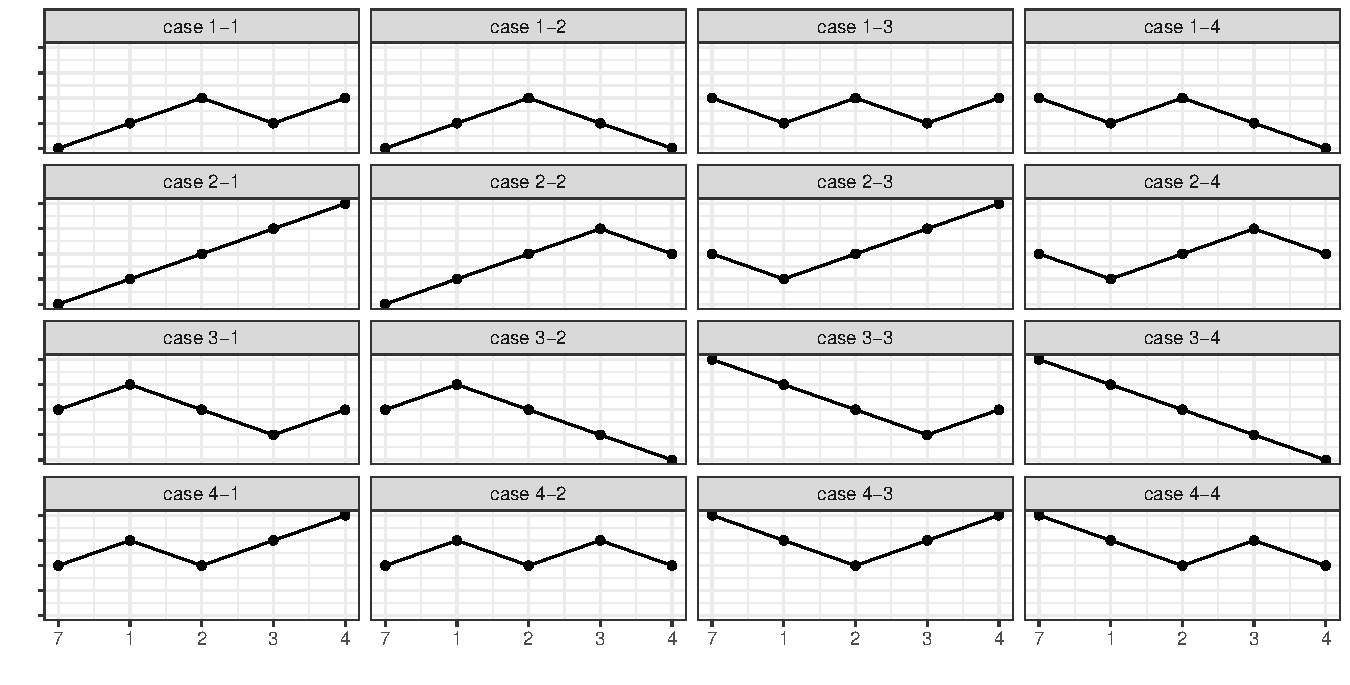
\includegraphics[width=1\textwidth]{Fig1.pdf}
\caption{가능한 지형들의 경우들}
\end{figure}
\dash

\para{주장3}: $\tau=\ell-1$에서 성립한다면 $\tau=\ell$에서도 성립한다. 

\para{주장3의 증명:}
\ck 지형의 모양은 모두 4가지 경우가 있다. 
(1) 로칼맥시멈 (2) 우상향 (3) 좌상향 (4) 로칼미니멈 
\ck 아래를 보이면 된다. 
\[
\Sigma_{13}^{\ell}-\Sigma_{12}^{\ell}=\Sigma_{13}^{\ell-1}-\Sigma_{12}^{\ell-1}+(h_{1}^{\ell}-h_3^{\ell})^2-(h_{1}^{\ell}-h_2^{\ell})^2\geq 0
\]
그런데 $\Sigma_{13}^{\ell-1}-\Sigma_{12}^{\ell-1}>0$ 이므로 아래를 보이면 충분하다. 
\begin{align*}
& A:=(h_{1}^{\ell}-h_3^{\ell})^2-(h_{1}^{\ell}-h_2^{\ell})^2 \\
& =(h_1^{\ell-1}+\xi_{1}^{\ell}-h_3^{\ell-1}-\xi_3^{\ell})^2-(h_1^{\ell-1}+\xi_{1}^{\ell}-h_2^{\ell-1}-\xi_2^{\ell})^2 \\ 
& =(h_1^{\ell-1}-h_3^{\ell-1})^2+(\xi_1^{\ell}-\xi_3^{\ell})^2-2(h_1^{\ell-1}-h_3^{\ell-1})(\xi_1^{\ell}-\xi_3^{\ell}) \\
&\quad - (h_1^{\ell-1}-h_2^{\ell-1})^2-(\xi_1^{\ell}-\xi_2^{\ell})^2+2(h_1^{\ell-1}-h_2^{\ell-1})(\xi_1^{\ell}-\xi_2^{\ell})\geq 0
\end{align*}
그런데 
\[
(h_1^{\ell-1}-h_3^{\ell-1})^2-(h_1^{\ell-1}-h_2^{\ell-1})^2 \geq 0 
\]
이므로 아래만 보이면 된다. 
\[
(\xi_1^{\ell}-\xi_3^{\ell})^2-2(h_1^{\ell-1}-h_3^{\ell-1})(\xi_1^{\ell}-\xi_3^{\ell})-(\xi_1^{\ell}-\xi_2^{\ell})^2+2(h_1^{\ell-1}-h_2^{\ell-1})(\xi_1^{\ell}-\xi_2^{\ell})\geq 0
\]
아래와 같이 나누자. 
\[
\textcolor{orange}{A_1:=(\xi_1^{\ell}-\xi_3^{\ell})^2-(\xi_1^{\ell}-\xi_2^{\ell})^2}
\]
\[
\textcolor{orange}{A_2:=-2(h_1^{\ell-1}-h_3^{\ell-1})(\xi_1^{\ell}-\xi_3^{\ell})+2(h_1^{\ell-1}-h_2^{\ell-1})(\xi_1^{\ell}-\xi_2^{\ell})}
\]

\ck 먼저 $\ell-1$시점에서 블락된 경우를 고려하자. 블락되고 노드 1에 왔다면 $A_1=0$ 이다. 따라서
\[
A=A_2=2b\left(h_3^{\ell-1}-h_2^{\ell-1}\right)
\]
블락된 이후 노드2로 왔다면 $A_1=-b^2$ 이고 
\[
A=-b^2+A_2=-b^2+2b(h_1^{\ell-1}-h_2^{\ell-1})=2b\left(h_2^{\ell-1}-h_1^{\ell-1}-\frac{b}{2}\right)
\]
블락된 이후 노드3으로 왔다면 $A_1=b^2$이고 
\[
A=b^2+A_2=b^2+2b(h_1^{\ell-1}-h_3^{\ell-1})=2b\left(h_1^{\ell-1}-h_3^{\ell-1}+\frac{b}{2}\right)
\]
블락된 이후에 각 경우에 대하여 평균적으로 $A$는
\[
2b\left( h_3^{\ell-1}-h_2^{\ell-1}+h_2^{\ell-1}-h_1^{\ell-1}-\frac{b}{2}+h_1^{\ell-1}-h_3^{\ell-1}+\frac{b}{2}\right)=0
\]
이는 지형에 상관없이 성립한다. 따라서 블락된 경우는 따질 필요가 없다. 

\ck $\ell-1$ 시점에서 형성된 지형의 조합수는 무한하다. 하지만 그림1과 같은 경우로 요약할 수 있다. 


\ck $\ell$ 시점에서 눈이 쌓이는 경우는 아래의 경우가 있다. 
\begin{itemize}
\item $(\xi_1^\ell,\xi_2^\ell,\xi_3^\ell)=(0,0,0) \Longrightarrow A=0:=a_0$
\item $(\xi_1^\ell,\xi_2^\ell,\xi_3^\ell)=(\tilde{b},0,0) \Longrightarrow A=2\tilde{b}(h_3^{\ell-1}-h_2^{\ell-1}):=a_1$ 
\item $(\xi_1^\ell,\xi_2^\ell,\xi_3^\ell)=(0,\tilde{b},0) \Longrightarrow A=2\tilde{b}\left(h_2^{\ell-1}-h_1^{\ell-1}-\frac{\tilde{b}}{2}\right):=a_2$
\item $(\xi_1^\ell,\xi_2^\ell,\xi_3^\ell)=(0,0,\tilde{b}) \Longrightarrow A=2\tilde{b}\left(h_1^{\ell-1}-h_3^{\ell-1}+\frac{\tilde{b}}{2}\right):=a_3$
\end{itemize}
\note $a_1+a_2+a_3=0$임에 유의할것. 
\ck cases 2에 해당하는 경우들을 따져보자. $\Xi_{\bullet 1}$
\[
C_i=\big\{\bs{\Xi}^\ell:\xi_i^{\ell-1}>0 \big\}
\]

\parared{case 1-1 $\sim$ 1-4} 
\ck cases 1-1의 경우 (7번노드) $A=0$ (1번노드 )
\one $A=0$
\two $A=\frac{a_1+a_3}{2}$
\three block 
\four $A=\frac{3a_3}{4}$
\ck 따라서 $\frac{5a_1+2a_3}{4}$

\parared{1-2} 
\seven $A=0$
\one $A=0$
\two $A=\frac{a_1+a_3}{2}$
\three $A=0$
\four $A=0$
\ck 따라서 $\frac{2a_1+2a_3}{4}$.

\parared{1-3} 
\seven $A=\frac{3a_1}{4}$
\one block
\two $A=\frac{a_1+a_3}{2}$
\three block
\four $A=\frac{3a_3}{4}$
\ck 따라서 $\frac{4a_1+4a_3}{4}$.

\parared{1-4} 
\seven $A=\frac{3a_1}{4}$
\one block
\two $A=\frac{a_1+a_3}{2}$
\three $A=0$
\four $A=0$
\ck 따라서 $\frac{5a_1+2a_3}{4}$.

\ck 경우1을 종합하면 $\frac{16a_1+10a_3}{4}$

\parared{4-1} 
\seven $A=0$
\one $A=\frac{a_2}{2}$
\two block
\three $A=a_2$
\four $A=\frac{3a_3}{4}$
\ck 따라서 $\frac{6a_2+3a_3}{4}$

\parared{4-2} 
\seven $A=0$
\one $\frac{a_2}{2}$
\two block
\three $\frac{a_2}{2}$
\four $A=0$
\ck 종합 $\frac{4a_2}{4}$

\parared{4-3} 
\seven $A=\frac{3a_1}{4}$
\one $A=a_2$
\two block
\three $A=a_2$
\four $A=\frac{3a_3}{4}$
\ck 종합 $\frac{3a_1+8a_2+3a_3}{4}$

\parared{4-4} 
\seven $A=\frac{3a_1}{4}$
\one $A=a_2$
\two block
\three $A=\frac{a_2}{2}$
\four $A=0$
\ck 종합 $\frac{6a_2+3a_3}{4}$

\ck 경우4를 종합하면 $\frac{3a_1+18a_2+9a_3}{4}=\frac{16a_2+6a_3}{4}$
\ck 경우1과 경우4를 종합하면 $\frac{16a_1+10a_3}{4}+\frac{16a_2+6a_3}{4}=\frac{16a_1+16a_2+16a_3}{4}=0$

\ck 따라서 각경우가 존재할 확률이 같다는 것만 증명하면 끝난다. 

\dash 

\dash

\ck 다른연습장 
\ck $\ell$-시점에서 눈이 빨강상태에 있다고 하자. 즉 $\xi^{\ell}(v_1)>0$. 그리고 $\ell+N_{1,7}^{\ell}$시점에서 보라에 있다고 하자. 즉 $\xi^{\ell+N_{1,7}^{\ell}}(v_7)>0$. 아래가 성립함을 주장할 수 있다.
\[
\mbox{for all $i, j$: } N_{i,j}^{0}=N_{i,j}^{1}=N_{i,j}^{2}=\dots
\]
따라서 그냥 아래와 같이 쓰자. 
\[
N_{i,j}
\]
이때 $N_{i,j}$는 노드 $i$에서 출발하여 $j$로 도착한 횟수이다. 이것을 hitting time이라고 하자. 

\ck unweighted regular graph의 경우 아래가 존재한다. 
\[
N^*=\min_{i,j} N_{i,j}
\]
따라서 아래도 존재한다. $E(N^*)$도 존재한다. 구체적으로 $E(N^*)=\frac{1}{\sum_{j}^{n}E_{1j}}$이다. 그리고 임의의 두 노드사이의 hitting time의 평균 즉 $EN_{i,j}$은 $EN^*$의 배수로 표현가능하다. 

\subsection{링과 링이 아닌 그룹은 분리할 수 있다.}
\dash 


\end{document}

